\documentclass[]{report}
\usepackage{graphicx}
\usepackage{todonotes}	
\usepackage{booktabs}
\usepackage{listings}
\usepackage[margin=1in]{geometry}
\usepackage{float}
\graphicspath{{resources/images/}}
\setcounter{secnumdepth}{5}



% Title Page
\title{Utilising peer-to-peer networking for data transfer over the browser}
\author{
	 Dominic Rathbone
	 \\ Student Number: 12843140 
	 \\ BSc Computer Science 
	 \\ Git Repository \& Documentation available: 
	 \\	https://github.com/domr115/CI301-Final-Year-Project 
	 }


\begin{document}
\maketitle
\tableofcontents

\chapter{Project Scope}
\section{Aims and Objectives}
	The ultimate objective of the project is to investigate the plausibility of data transfer over web browsers (in particular, file transfer and media streaming) without the need for a centralised client-server architecture, instead opting for a peer-to-peer network architecture. To achieve this, the plan is to:
	\begin{itemize}
		\item Research peer-to-peer networking architecture and topologies.
		\item Research current solutions to file transfer over the browser.
		\item Research WebRTC.
		\item Develop a session signalling server in Java with the WebSockets protocol
		\item Develop a WebRTC Application to transfer and stream uploaded files.
		\item Implement a structured peer to peer network between peers transferring/streaming a file using the web application.
	\end{itemize}
\section{Stakeholders}
	The stakeholders involved in the project will be myself, my supervisor, Stelios Kapetanakis and the user.
\section{Methods of Communication}
	As stakeholders, we have set up a regular weekly meeting to catch up on what has been achieved that week. On top of this, we communicate regularly via email and Skype. Stelios also has access to a GitHub repository containing the project and a work flow board hosted on a personal web server to track the progress of the project. 
	
\chapter{Research}
	
	\section{Current Solutions to Data Transfer}
	Currently, solutions such as DropBox and Google Drive focus on cloud storage as a service whilst providing the ability to transfer data as a secondary function of this. Although this is an extremely valuable and convenient idea enabling consumers to back-up their data, not all want a third party service that stores the data they want to transfer as this does raise ethical issues, namely with the data's security, privacy and ownership once it has been uploaded. However as a consumer, this can be hard to avoid when the online storage and transfer of data are so closely coupled and these services have a huge market share.
	
	Once a user has uploaded files to one of these services, there is a trust placed on the company to store the data securely. However it could be argued that this trust is often misplaced, for example in 2010 the "Cloud Security Alliance" released a regularly updated list of the top threats faced by cloud computing services suggesting there are numerous security issues faced within the cloud computing industry with many of the issues on this list occurring due to malicious intentions. For example the 6th item on the list, "Malicious Insiders" describes a situation in which current or former employees abuse their credentials within the system to gain access to sensitive information \cite{CSA Top Threats}. This suggests that even though companies can protect their client's data from outsiders to an extent, there are still issues such as this that the industry face and consumers may want to avoid.
	
	Whilst the uploaded data can be encrypted in a way that means only clients of the service can decrypt it (through end-to-end encryption), many people feel insecure leaving traces of their private information on a remote server belonging to a company that is not necessarily always acting in their interest. In 2013, this concern was legitimized by Edward Snowden when he disclosed information about government surveillance programs such as PRISM that coerced firms such as Google, Microsoft and Yahoo to provide private consumer data from their services to the government \cite{PRISM}. More recently, this idea has been reinforced by legislation such as the "Investigatory Powers Bill" being introduced in the UK that could prohibit companies from using end-to-end encryption techniques, allowing authorities to request decrypted client data \cite{IPB Encryption}. Whilst we can assume they have done this with non-malicious intentions, by weakening the encryption practices of these companies, they also weaken the defence against malicious attackers.
	
	As an alternative to using cloud storage solutions for sharing files, there is also specific data transfer sites such as WeTransfer that allows you to send files of sizes up to 2 gigabytes via their application which works by sending a link through email to the target recipient. Whilst it does store the uploaded files, they are only kept for 7 days in order to prevent unnecessary storage costs \cite{WeTransfer Storage Time}. Although this is better for data privacy, WeTransfer use third party providers such as Amazon Web Services (AWS) to store this data using AWS S3 Storage \cite{WeTransfer AWS Case Study} meaning there is still the potential concern of data privacy and security highlighted previously. Amazon in particular, has been exposed for how easily it's customer service can be socially engineered \cite{Amazon Social Engineering}
	
	Peer-to-peer networks have also been popular for file sharing since the late 1990s due to the rise of applications such as Napster which focused on music sharing via peer-to-peer . Napster worked by using a central server to index files that each peer makes available on their machine. Each peer would then be able to search the index for copies of songs and download them from each other. However, this service was eventually shut down as the company ran into legal problems with copyright infringement. Since then, protocols such as BitTorrent have improved on the idea of peer to peer sharing. The BitTorrent protocol works by peers creating ".torrent" files that describe the file's metadata, this is then shared however it is seen fit, normally via torrent websites. Each peer wanting to download this file then picks up this ".torrent" file, opens it with a BitTorrent client and joins a "swarm" of peers, becoming one of the many "leechers" downloading this file. At the same time, this peer becomes one of the many "seeders" uploading this file as they download it so that other leechers can also download it from them. The initial peer discovery is based on "trackers", servers hosting lists of seeders and leechers for the file. One of the issues with BitTorrent is that in order to share a file, you must go through the process of downloading a client, creating a ".torrent" file, adding it to a trackers list and sharing the ".torrent" with your peers and this can be seen as a arduous task for a basic consumer looking to share their files. Another problem is that if a tracker server is compromised, there is potential for malicious attacks using the information stored on it.
	
	As an alternative to these current solutions, the application I plan to develop has the aim of separating the online transfer of data from it's storage by connecting the peers involved in the transfer directly with each other. This circumvents the problems with cloud storage as the data being transferred does not pass through any servers as well as some of the problems with current peer to peer file sharing as it does not require a desktop client or torrent files. To allow my application to share files online, a technology called WebRTC will be used.
	
	\section{Comparing Network Architectures}	
	Peer-to-peer networking is the distribution of resources and processing between a set of nodes in a network. These tend to take the form of an overlay network which is an architecture describing a virtual network that sits on top of a physical network (e.g the internet) and consist of a subset of the nodes connected to this physical network.
	
	\begin{figure}[H]
		\caption{
			An Unstructured Peer-To-Peer Overlay Network 	
			\cite{Unstructured P2P Diagram}
		}
		\centering
		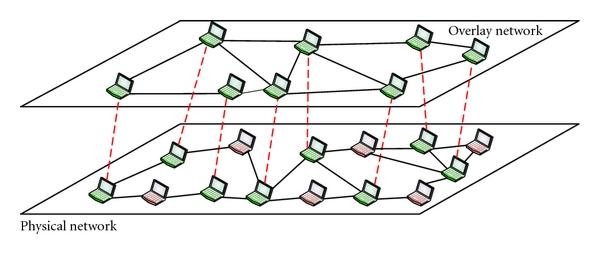
\includegraphics{overlaynetwork.jpg}
	\end{figure}
	
	Although an overlay network does not need to manage the burden the physical network is responsible for such as low level communications protocols. it does need to manage things such as peer discovery and management. There are several different architectures defining how a network can do this:
	
	\begin{itemize}
		\item Unstructured peer-to-peer:
		Peer connections in the overlay network are established randomly and do not adhere to a topology. New peers copy the connections a previously established peer has formed and randomly develops it's own over time.\cite{P2P overlay networks}. These networks are easier to build than structured networks as routing is random and does not require management. They also tend to fair better in periods when the rate of peers leaving and joining (or churn rate) is high due to this non-deterministic nature. However, searching in these networks tends to be less efficient as they rely on flooding the network to find nodes that hold the data they are searching for.
		\item Structured peer-to-peer:
		Peers in a network are organised in a stricter network topology and use a specific protocol to manage and discover peers. An example of one of these protocols is using a distributed hash table to share data over a network. This table is distributed amongst the peers of the network, each of them holding unique keys generated from hashing parts of the data they have got. To maintain this, peers hold a routing table which link it to other peers containing parts of the hash table. In order to for a peer to get the parts of the data they need, they are able to either get it from a neighbour or route through to a different peer through that neighbour in order to get closer to it \cite{P2P overlay networks}. 
		\item Hybrid peer-to-peer:
		These networks involve the use of centralized servers in some way, how it does so is determined by the implementation details. This model tends to work better than both unstructured and structured as features that function better in decentralized networks can be left to the peers in the network whilst the server can handle the features it is more efficient at. However, this architecture can be liable to scaling and redundancy issues due to the dependence on a server. \cite{Hybrid P2P network}.
	\end{itemize}
				
	In contrast to peer-to-peer networking, there is also the client-server model. In a basic sense, this is when the machines processing or storing data (servers) are distinct from the computers using this data (client). Although in actuality, the boundaries between them vary dependent on how the model is implemented. Whilst the shift of processing on to a server means that the user of an application does not need a powerful machine to run it, it also means that the application supplier has the responsibility of maintaining and paying for these servers. Furthermore, although modern server architectures are designed in a distributed structure granting them to be more robust (as distribution allows for scaling and redundancy), if these servers undergo too much load or in extreme cases, if the server farm completely crashes, the user would not be able to run the application as intended.
	
	Using a peer-to-peer architecture avoids the issues associated with the client-server model as processing is distributed between the nodes making up the network, resulting in it being cheaper to maintain as there is less reliance on servers and more robust as the network scales as more peers join and load increases. However, there are a number of considerations to be aware of in peer-to-peer networking, the largest being security as there is no centralized authority to manage access control to resources. Thus, a malicious client could join a network and potentially launch a number of attacks versus other nodes within it such as Denial Of Service where a malicious group of nodes floods a network with a massive amount of fake requests, potentially crashing nodes within it or Man in the Middle  attacks where a node is able to intercept data flowing between two other nodes and spy on or poison it\cite{P2P Security Issues}. Whilst it would be difficult to completely avoid risks like this as it is an inherent flaw in peer-to-peer architectures, introducing the basic concept of trust into a peer-to-peer network can stop malicious peers from entering it in the first place. This could be implemented in the application by allowing users to enable authentication (via password) for the uploaded file potentially preventing malicious attackers from being able to access the room to download or stream it. 
	
	The application will most closely resemble a hybrid peer-to-peer network as even though the actual channel for transferring data between peers will not go through a server, one will be used for the process of signalling to route peers together. To form a network of peers that go beyond a one-to-one peer connection, the signalling server in conjunction with the client-side application will have to manage how these peers connect to each other. This is known as a network's topology and one way of modelling it is a line network where a peer joins the network and connects to one other peer which is in turn, also linked to the peer that it connected to when it joined and so forth, forming a linear chain of peers that can reroute if a neighbouring peer disconnected.
	
	\begin{figure}[H]
		\centering
		\caption{Linear network}
		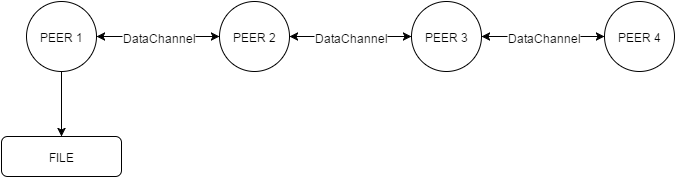
\includegraphics[scale=0.4]{network.png}
	\end{figure}
	
	\begin{figure}[H]
		\centering
		\caption{Peer disconnects from the network}
		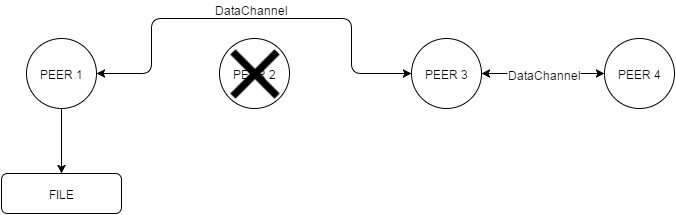
\includegraphics[scale=0.4]{peerdisconnect.png}
	\end{figure}
	
	However, this would become inefficient if a peer in the chain malfunctioned or restricted bandwidth without disconnecting, potentially bottlenecking the rest of the peers behind it. As an alternative, peers could be routed based on a tree network topology \cite{Tree Topology} consisting of "super-nodes", high capability peers that relay the transferred data to sub-nodes. This way load can be balanced across many nodes by distributing new ones to another super-node or by electing further super-nodes if the load increases too much or if one disconnects. By exploiting heterogeneity between peers of the network, this topology can also be used to improve it's performance by electing super-nodes based on criteria such as location and, in our case, how much of the data has already been transferred or streamed to them. By doing so, performance within a network can potentially be improved as sub-nodes can be connected to super-nodes based on this criteria, e.g if a sub-node is located in the same place as a super-node then use it.\cite{Supernodes}.		
	\begin{figure}[H]
		\centering
		\caption{Tree Network}
		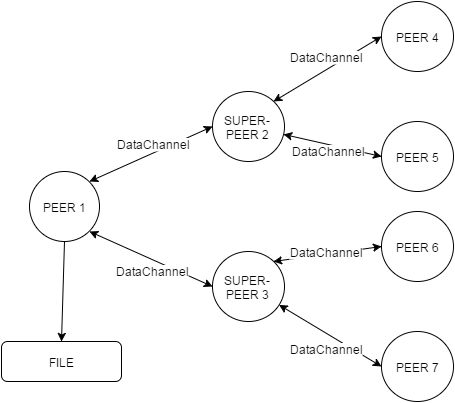
\includegraphics[scale=0.4]{treetopology.png}
	\end{figure}			
	
\section{WebRTC}			
	WebRTC (Real Time Communication) is an emerging web technology that enables browsers to communicate in real-time via a peer-to-peer connection, avoiding the need for a centralized server to transfer data between clients. This was first released by Google as an open source project in May 2011 \cite{Google WebRTC Release} and was later drafted as an API definition by W3C, remaining as a work in progress. \cite{W3C WebRTC Definition}. WebRTC has yet to be fully implemented in every web browser but Chrome, Firefox and a WebRTC specific browser called Bowser do support it. Firefox (Nightly) in particular seems to be leading the way in this field and so the application will specifically be developed towards this browser\cite{WebRTC browser support}.
	The 3 main WebRTC APIs supported at this time are:
		\begin{itemize}
			\item RTCPeerConnection:
			"The RTCPeerConnection interface represents a WebRTC connection between the local computer and a remote peer. It is used to handle efficient streaming of data between the two peers." \cite{Mozilla Web API}
			\item RTCDataChannel:
			"The RTCDataChannel interface represents a bi-directional data exchange channel between two peers of a connection." \cite{Mozilla Web API}
			\item getUserMedia:
			"Prompts the user for permission to use one video and/or one audio input device such as a camera or screensharing and/or a microphone. If the user provides permission, then the successCallback is invoked with the resulting MediaStream object as its argument. If the user denies permission or media is not available, then the errorCallback is called with PermissionDeniedError or NotFoundError respectively. Note that it is possible for neither completion callback to be called, as the user is not required to make a choice."\cite{Mozilla Web API}. Note, this is not actually a part of the WebRTC API, rather the Navigator API but is still necessary to use it.
		\end{itemize}
		
	In order to achieve it's aim, the application will utilize the RTCPeerConnection and RTCDataChannel APIs. The former to establish a peer connection between two clients and to stream media files whilst the latter will be used to create a channel over this peer connection to transfer data.
			
	As shown by the Javascript Session Establishment Protocol (JSEP) \cite{JSEP}, although WebRTC and the browser is used to transfer the data between two peers, it purposely does not handle the protocol signalling occurs over. Signalling is a concept that came from telecommunications and VoIP and is the process of organising the communication between two clients, handling the exchange of metadata that creates and manages a session. The rationale behind WebRTC being signalling-agnostic is that different applications will require particular protocols in order to be able to fit into previously existing architecture or meet a specific requirement regarding the protocols used. However to use WebRTC, the signalling protocol must be able to support duplex communication to send messages over.
	
	\begin{figure}[H]
		\caption{WebRTC Architecture as defined by JSEP \cite{JSEP}}
		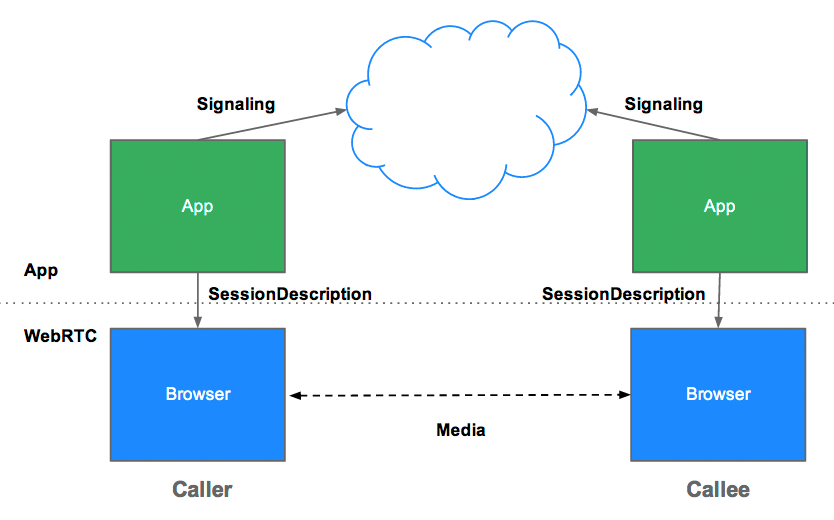
\includegraphics[scale=0.4]{jsep.png}
	\end{figure}
	
	WebSockets is a protocol implemented by browsers and servers to provide bi-directional communication between them\cite{WebSockets}. Once established, a session is left open for the server to send messages to the client and vice versa, making it a good candidate for signalling with a WebRTC application which needs peers to be able to reliably send messages back and forth through the server. Over this WebSockets session, SDP signals will be sent. SDP is a communication protocol that specifies how signals are modelled \cite{SDP Over WebSockets}. As a convenience, most browser implementations of WebRTC handle the generation of these SDP signals. To establish a connection, one peer sends an offer SDP to another through the signalling server, the receiving peer generates an answer SDP which is sent back, forming the connection. To get the peer's location, WebRTC uses a process called interactive connectivity establishment (ICE) to find a list of the possible IP's and ports of each peer which are then sent through the signalling channel. Once this is done, a data channel or a media stream can be added to the connection to either transfer or stream data. For streaming, WebRTC secures these packets of data by Secure Real Time Transport Protocol (SRTP) and for the data channel, the packets are secured by Stream Control Transmission Protocol (SCTP) and encrypted by Datagram Transport Layer Security (DTLS) \cite{WebRTC Data Channel Establishment Protocol}. 
	
	\begin{lstlisting}[tabsize=1,frame=single, basicstyle=\ttfamily\footnotesize]

	\end{lstlisting}
				
\chapter{Specification}
	\section{Deliverables}
	The first intermediate product will be the signalling server written in Java. This will handle the exchange of client meta data in order to establish the connection between two peers using the web application. The development of this is overlapped with the development of the data transfer functionality and user interface of my second deliverable, the web application to make manual testing of the signalling server significantly easier.
	
	The first end deliverable will be the client side web application the user interacts with in order to select a file as well as handling sending the meta data to the signalling server and managing the peer-to-peer data transfer and media streaming. This is broken down into several intermediate products, the data transfer functionality, the media streaming functionality, the peer-to-peer network and the user interface. I plan to produce the data transfer functionality first along side the user interface to allow for manual testing. After I have implemented data transfer, I will work on media streaming and forming the peer-to-peer network topology. 
	
	The second end deliverable will be the final report containing documentation and analysis using the metrics from my application, comparing how it and technologies behind it perform in comparison to others, focusing in particular on how peer-to-peer over the browser (WebRTC) compares to other methods of data transfer and media streaming.
	
	\newpage
	\begin{figure}[h!]
		\caption{Schedule of Activities}
		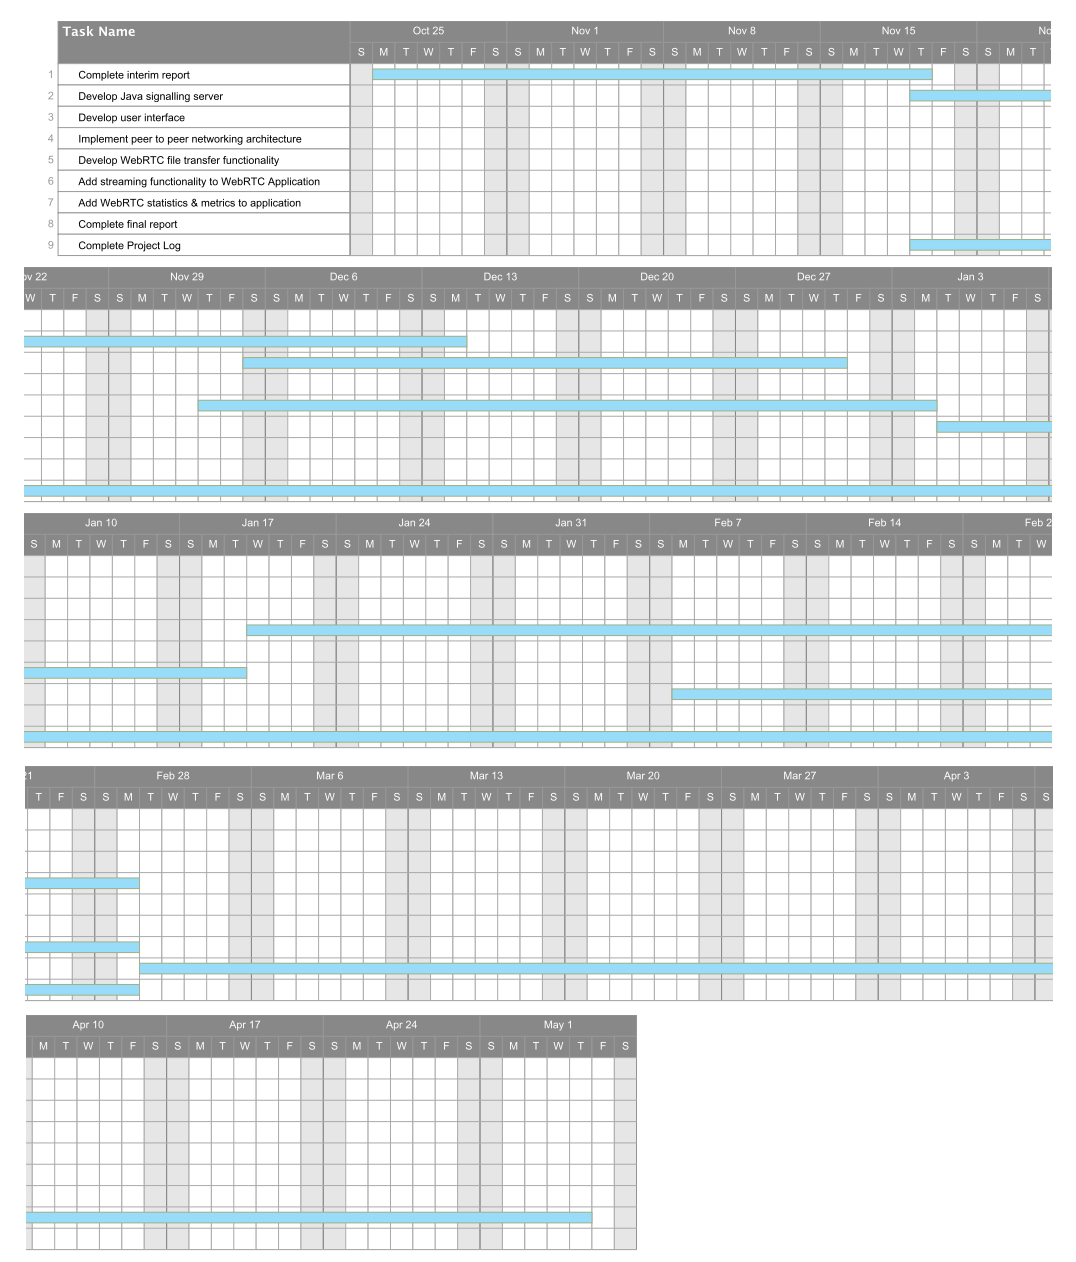
\includegraphics[scale=0.5]{ganttchart.png}
	\end{figure}
	\newpage	
	
\section{Risk Analysis}
	\scalebox{0.6}{
		\begin{tabular}{@{}|l|l|l|l|l|@{}}
			\toprule
			\textbf{Risk}                                      & \textbf{Probability (1-5)} & \textbf{Impact (1-5)} & \textbf{Mitigation}                                                                                                  & \textbf{Contingency}                                                                            \\ \midrule
			Illness/Injury                                     & 4                          & 3                     & \begin{tabular}[c]{@{}l@{}}Reserve time for illness\\ Be hygienic\\ Eat healthy\\ Exercise\end{tabular}              & \begin{tabular}[c]{@{}l@{}}Allow time for recovery\\ Take medicine to aid recovery\end{tabular} \\ \midrule
			Inaccurate estimations                             & 3                          & 3                     & \begin{tabular}[c]{@{}l@{}}Be liberal with estimations\\ Reserve time for deliverables behind schedule\end{tabular}  & Adjust scope of project                                                                         \\ \midrule
			Data loss                                          & 1                          & 5                     & \begin{tabular}[c]{@{}l@{}}Use a version control system\\ Keep local backups\end{tabular}                            & Recover data from Git                                                                           \\ \midrule
			Uncommunicative stakeholder                        & 1                          & 3                     & Ensure regular meetings with stakeholder                                                                             &                                                                                                 \\ \midrule
			Stakeholder turnover                               & 1                          & 4                     & N/A (out of my control)                                                                                              & Get new stakeholders                                                                            \\ \midrule
			Project scope too large                            & 3                          & 4                     & \begin{tabular}[c]{@{}l@{}}Research enough to be certain in project scope\\ Be liberal with estimations\end{tabular} & Adjust scope of project                                                                         \\ \midrule
			Technologies too immature/insufficient for project & 2                          & 4                     & Research technologies beforehand                                                                                     & \begin{tabular}[c]{@{}l@{}}Find alternative technologies\\ Adjust scope of project\end{tabular} \\ \bottomrule
		\end{tabular}
	}

	\section{Quality Analysis}
	The main measure of success will be the web application's performance in it's ability to transfer \& stream data between two peers. To track this, I will implement metrics using the WebRTC "getStats" statistics API, which allows for monitoring of the bandwidth usage, packets lost and network delay within a connection between two peers. I will then gather these statistics in two different cases, one where there is no formal network structure (to find a baseline) and then when the many-to-many network has been implemented to compare if the structured peer-to-peer network does improve performance of the application. This network will also have it's own monitoring to ensure that peers are being correctly organised. Further to this, I will also compare the speeds of file transfer with other services such as DropBox through their API, however this may prove unrealistic as these services will be running on more powerful servers. To certify that the user-experience is acceptable, the application will also be user-tested. The signalling server will be load tested in isolation to make certain it can handle multiple requests to ensure it does not bottleneck the application. 
			
	\chapter{Methodology}
	I chose to use an alternative methodology to the waterfall model because it lacks the ability to adapt to changes throughout a project's timeline. Due to the way waterfall is structured into different phases that must be completed sequentially, often when changes such as new requirements occur, all these phases must be repeated in order to account for it.	Thus, as a way of managing this project, I plan to use an iterative and evolutionary methodology. . Iterative methodologies take an approach that can adapt to these changing requirements because they utilise short development cycles and focus on developing small modules of a product at one time, making it easier to revise one if necessary. This is particular useful in this project as it is relatively experimental and the requirements may change regularly. Whilst it will be similar to processes such as scrum, it will not have the stricter framework surrounding it that requires a product owner and scrum master. This methodology will be relatively simple and based around a backlog of tasks from which a developer takes from in a limited amount, normally one to two tasks at a time which are then pushed through the work flow.
		
	In my case, the work flow will be relatively simple:
	\begin{enumerate}
		\item To Do
		\item In Progress
		\item Code Review
		\item Manual Testing
		\item Done
	\end{enumerate}
		
	During the "In Progress" step of the work flow, the test driven development (TDD) methodology will be used in which tests are written first and then the application is coded to pass the test. By doing so, this makes development a short iterative process and ensures that the code is only doing what it is supposed to, minimising side-effects and stopping bugs from occurring. However, this process will be fairly lenient and only used  on parts of the code that require stringent testing as writing tests for things such as boilerplate code is unnecessary and will take up development time. 
	
	\begin{figure}[H]
		\caption{
			Test-Driven Development (TDD) Cycle
			\cite{TDD Diagram}
		}
		\centering
		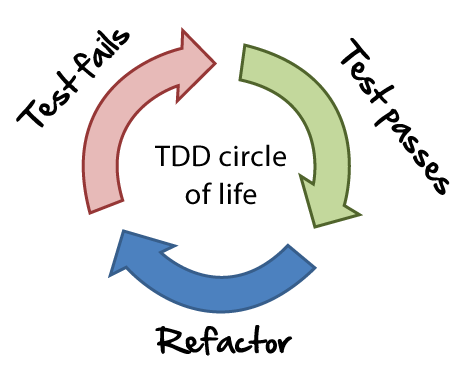
\includegraphics[scale=0.5]{tdd-circle-of-life.png}
	\end{figure}
	
	During the "Code Review" step, the development task will be self-evaluated to ensure the code follows conventions. On top of this, I will run static code analysis tools (such as FindBugs/PMD for Java) and use the code review section StackExchange to get second opinions if a task is found to be particularly difficult. If it passes the code review step and it is possible to do so, the task will also be black-box tested from a user's perspective to see that it actually works as intended. Once every task forming a feature is completed, the feature will be manually tested as a whole to see that each task has integrated together as planned.
	
	To visualise this workflow, the open source web application "Kanboard" hosted on an Amazon Web Instances EC2 Instance will be used. This will allow for the stakeholders to keep track of the progress throughout the duration of the project. To manage the actual changes made to the project files, the git version control system will be used in conjunction with a remote repository held on GitHub. The benefits of using version control is that it keeps the code base safe and logs every code commit as well as allowing for it to be worked on by multiple developers and on multiple devices. 
	
	\chapter{Development}
		\section{Architecture}
			\begin{figure}[H]
				\caption{Application Architecture}
				\centering
				\includegraphics[scale=0.5]{application-architecture.png}
			\end{figure}
			To organise the client-side application, each layer of JavaScript was developed in individual modules, separated by their responsibilities. These layers consisted of the main application module serving as the entry point into the code and had the responsibility of listening to and manipulating the document object model, the peer-to-peer module which uses WebRTC to establish the peer connections and the signalling module that established the WebSocket connection. By separating these layers into their own modules, the application was left with a relatively simple architecture that can easily be refactored and extended without causing side-effects in other modules.
			
			In order to manage these modules and their external and internal dependencies, a build tool called Browserify was used. Traditionally, all of the JavaScript files are added via script elements within the html document they are associated with. Instead, this tool allows for a JavaScript file to be included as a dependency by using JavaScript. It does this by using the "require('module')" function to simulate the modular structure Node.js uses. This modular structure makes it clear which dependencies each module requires and provides a consistent way of doing so. Each JavaScript file is wrapped in a global function which Browserify can then export and bundle together into one larger JavaScript file using a command line interface. This bundled file is then referred to in the main HTML document. By organising JavaScript this way, Browserify enables the client side JavaScript to also use node modules, making full-stack development more efficient.
			
			The Node.js server uses the Express.js web framework for two purposes, to serve files to the browser by resolving URLs to static resources and to also provide the API which the client-side JavaScript application communicates with by routing HTTP requests to functions in the main server file. To support the bi-directional communication necessary for the two clients to talk, both the server and the client uses the Socket.io library to establish WebSocket sessions. Due to the application's peer-to-peer nature, the resulting architecture could be considered to have a "fat client" as most of the processing is achieved on the client side with the server-side functionality only functioning as a method of communications and organisation for them. Due to this, there was no need for more than one JavaScript module to model it's functionality. However in the future, if a feature such as the API is was expanded, it may need to be moved to it's own module. Overall, the dependence on a centralised server to organise the clients means the architecture of the application reflects that of a hybrid peer-to-peer network as defined in the research section.
				
			\begin{figure}[H]
				\caption{Application Flow Chart}
				\centering
				\includegraphics[scale=0.6]{application-flow.png}
			\end{figure}
			
			The diagram in Figure 5.2 shows how the applications transitions between each state within the application, \todo{FINISH}
		
		\section{Signalling}
			\subsection{1st Iteration - Spring Boot}
				\subsubsection*{Spring WebSockets Over STOMP}
				The first prototype of the signalling server for Transfer4me was implemented using Spring Boot. This is a part of the Spring application framework emphasising convention-over-configuration which is the idea that frameworks should supply a set of pre-configured technologies to be used by default as opposed to making the developer have to choose and configure them. This makes it a lot faster and easier to produce a working prototype. To support the WebSockets protocol, Spring uses the "STOMP" sub-protocol to model the message sent between server and client. STOMP is very similar to HTTP in how it models the message but is sent over TCP once the socket is established \todo{CITE}. Using the STOMP JavaScript client, an application can subscribe to several destinations and listen for events (by asynchronous callbacks) or publish events using a send method that takes a string identifying the event (which in this case is the "signal" event) and another string representing the message. The architecture that was created on top of this protocol used rooms that were created when a user uploads a file and were designated via a URL which the recipients then subscribe to when they load the page.

				To create these rooms, the client that uploads the file fires a request to the server using a HTTP endpoint. When the server receives this request, it generates a Room object and a UUID that serves as its identifier. This room is then added to a list and the ID is returned to the client in the response. The uploader then uses this ID to subscribe to the room over WebSockets. When this connection is established, the server creates a user object and adds it to the correct room. This ID is then appended to the base URL of the page for the uploader to share. The recipient loads the URL but only joins the room at the point at which it is necessary (when the recipient either chooses the download or stream button), this is a tactic called "lazy initialization" and by using it, the server only has to cope with the load from the WebSocket sessions that actually need to be connected as opposed to users that may be idle on the page.
							
				\subsubsection*{Problems}
				The main problem found with the Spring implementation was in it's limited functionality. It was extremely hard to implement sending messages to specific individual sockets which limited how multiple peer connections could communicate within the same room as they would all be receiving every signal being exchanged through it. This could be avoided to an extent by making each client application only pay attention to the messages that were destined for it by appending an identifier for the destination to each message but that would only stop the clients from using the messages as opposed to receiving them. As a result, this is not a viable solution as it leaves the application open to man-in- the-middle attacks because a user could easily modify the client-side application to log all of the messages that it received which is a major issue in this case as the majority of the messages sent will be WebRTC meta-data such as your IP address.
				
			\subsection{2nd Iteration - Node JS}
			To solve the problems found with the Spring implementation, the server was re-factored using Node.js as a replacement. This is a server-side JavaScript environment that uses an event-driven approach wherein the flow of the application is determined by continuously listening for and reacting to events via callbacks. This concept allows the environment to run asynchronously without having to employ multi-threading. As the client-side application was also written with JavaScript, using Node.js means the full-stack employed this language. This made the development process considerably easier as it meant time was not spent acclimatising to a different language when switching from working on the server to the client. As the code is no longer separated into two different languages, it also has the added benefit of being able to reuse modules of code on either the server or client.
				\subsubsection*{Socket.IO}
				Node.js maintains support for WebSockets through the Socket.IO library which offers extended functionality over it's Spring counterpart. Socket.io models communication using the concepts of name spaces and rooms where a name space is represented by the endpoint a socket connects to and rooms are channels within this that users can join and leave, allowing for communications to be separated without having to use multiple endpoints. By default, every socket that connects to a name space has it's own room which means Socket.IO could broadcast events to specific user's rooms solving the security issues that the Spring implementation had. As a result of this, the architecture of the server was slightly changed to reflect this new functionality as there was no longer a need to have an object to specifically represent a user. 
				
				\begin{figure}[H]
					\caption{Signalling establishment sequence}
					\centering
					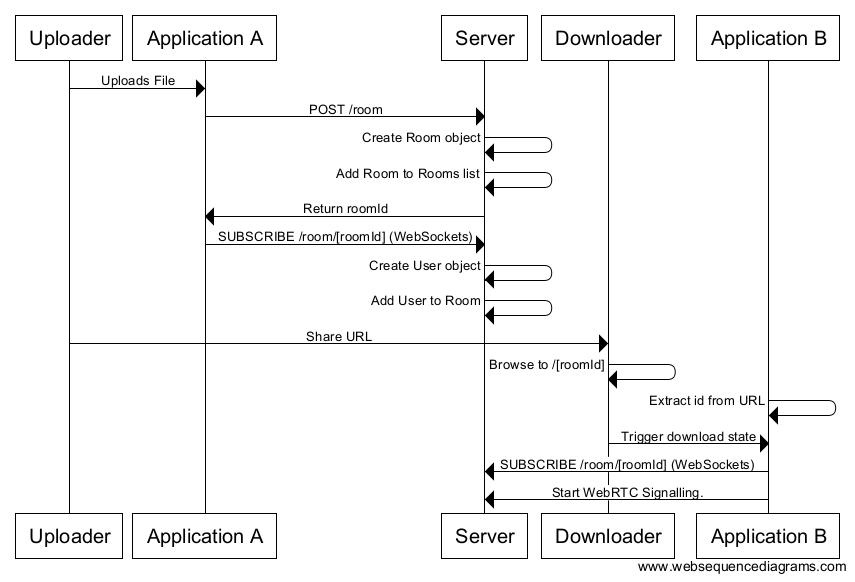
\includegraphics[scale=0.5]{signalling-establishment-sequence.png}
				\end{figure}
				
				\subsubsection*{API}
				After switching to Node.js, the API was extended to support new functionality in the client side web application. Another endpoint was added to retrieve the file type of the file uploaded as the application would previously let you select the stream option for any file (including files such as a text document) which evidentially caused failure. By adding this endpoint, it meant that the client-side application could retrieve the file type and only present the user with the corresponding options. It was also extended to allow the authentication process to work by modifying the current new room endpoint to generate a password if specified and adding a new endpoint to validate this password. 
				
				As these were added, it was realised that the API was becoming inconsistent and should be restructured in order to maintain uniformity amongst endpoints. As a result, the URI structure of each was re-factored using a RESTful approach. REST (Representational State Transfer) is an architectural style specifying that an endpoint into a system should be built around resources with methods for retrieving and manipulating this resource \todo{CITE}. In practice, these methods generally translate into HTTP verbs such as GET and POST. For example to add a room, a POST request is sent to the URI "/room" and to retrieve a room, a request is sent to "/room/{roomId}". These guidelines allow for an easily maintainable API as well as providing the client web application with a predictable and consistent group of endpoints to code against. As a RESTful API is modelled in terms of resources, it does not hold the state of a client's journey throughout the web application and thus, this is left up to the client consuming the resource which in this case is the JavaScript application. By doing so, it means the server is under less load and is in a better state to be scaled.
				
				\begin{description}
					\item [API Documentation]
				
					\item[POST /room] 
					Adds a unique room to the list of rooms on the server. Returns a JSON object containing a UUID for the room and, if the passworded field is present in the request body, a random string password.
						
					\item[GET /room/\{roomId\}/fileType] 
					Returns the MIME type of the file associated with the room.
					
					\item[POST /room/\{roomId\}/password] 
					Takes a password from the request body and compares it with the password associated with the room. If the password is correct, it will add a cookie containing the password to the response. If the password is false, it will return a 401 Unauthorized HTTP status code.
					
				\end{description}
				
				\subsubsection{JSON}
				Both the socket implementation and the API transfer data in a format known as JSON (or JavaScript Object Notation) in order to remain consistent throughout the application. This was chosen as the data transfer language because JavaScript has native functions for parsing to and from JSON as opposed to other common alternatives such as XML. JSON is also lot more human-readable than XML and the benefits of XML such as custom schema support was not necessary for this project.
		
		\section{Peer to Peer Communication}
			\subsection{One-to-one peer connection}
			As a starting point, I worked on using WebRTC to establish a simple peer connection between two clients. This process is achieved through negotiation using offers and answers representing what each client wants from the other client and what the client is willing to offer such as media streams and constraints. These parameters are modelled using a protocol called "Session Description Protocol" or "SDP" which is generated by WebRTC. In a traditional WebRTC architecture, the peer that sends the offer tends to have something to offer (such as a stream). However, the architecture for transfer4me is slightly different in this sense as the offer is sent from the recipient peer even though the uploader is the peer with the only peer with something to offer. This arises from how transfer4me uses WebRTC as a means to transfer files as opposed to its conventional purpose of establishing real-time communications. Due to this, the negotiation process is closer to reflecting the "request-response" pattern used in HTTP transactions more than it does an "offer-answer" model. This architecture also improves performance as the uploader does not have to send and maintain offers to every peer that joins the room which would eventually introduce a large amount of unnecessary load especially if the recipient peer joins but never downloads or streams the file. Instead, the offer is "lazily initialized" by the recipient peer in the sense it is only created and sent at the point it is needed which in this case is when they either opt to download or stream the file, this way the uploader only deals with the recipients that request the file. Once the offer SDP is created, it is stored as the local description and sent to the uploader via the signalling channel. The uploader receives this, sets it as the remote description and creates an answer SDP which is again set as their local description and sent back to the recipient via the signalling channel. Both these SDPs contain "ICE candidates" which detail potential IP addresses to be used to establish a connection. However, how WebRTC handles the retrieval of these ICE candidates depends on the browser as Chrome supports a concept called "trickle ICE" where ICE candidates can be sent on-the-fly as they are received regardless of whether the SDP has been sent or not whereas Firefox does not support this and all candidates have to be sent with the SDP. 
			
			\begin{figure}[H]
				\caption{Peer Connection Establishment Sequence in Chrome}
				\centering
				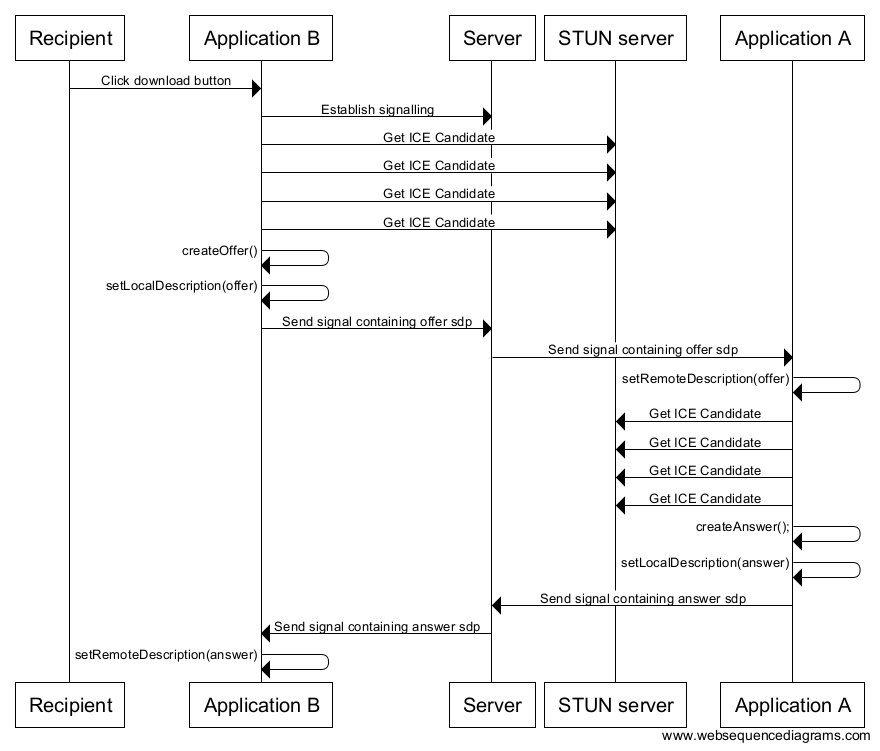
\includegraphics[scale=0.5]{peer-connection-establishment-sequence-chrome.png}
			\end{figure}
			
			\begin{figure}[H]
				\caption{Peer Connection Establishment Sequence in Firefox}
				\centering
				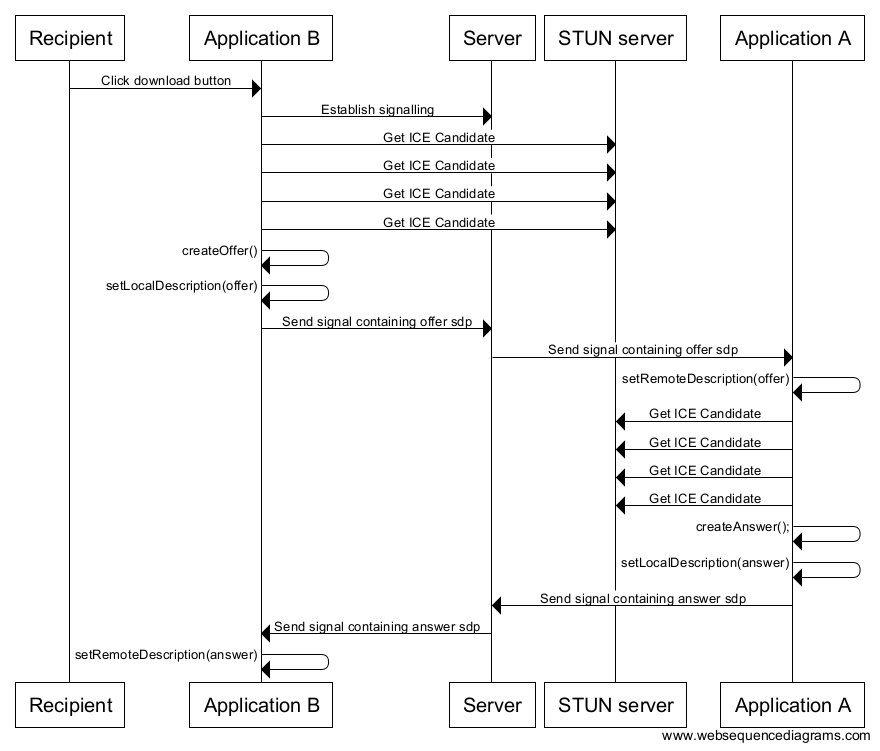
\includegraphics[scale=0.5]{peer-connection-establishment-sequence-firefox.png}
			\end{figure}
			
			\subsection{File Transfer}
			To upload a file, the application uses the HTML5 File API \todo{CITE} to retrieve the file from an input element which is then stored as a variable waiting to be sent to a recipient. In order to download the file, the recipient creates a new RTCDataChannel using the RTCPeerConnection API which is added to the offer to be sent to the uploader. Once the connection is established, the uploader waits for the addition and establishment of this RTCDataChannel via an asynchronous event listener. After this, how the file is sent depends on the browser. In Firefox, once the DataChannel reaches it's open state, a callback is fired which sends the file through. On the recipient peer's client, an event listener waits for messages to be sent through which then catches the file and saves it to the disk. However, Chrome's implementation of RTCDataChannel has a size limit on the messages that can be sent meaning the file has to be sliced into several smaller parts which can then by reassembled by the recipient (a process called chunking). The major problem with this approach is that it significantly bottlenecks how fast a file can be sent to the recipient in Chrome. Although this allows for cross-browser file sharing, sending files from Firefox to Firefox will always be faster for downloading via the application. Once this file has been received, it is then saved to disk by reading the file in as a data URI and then appending an element to the html with this URI as the reference. An automated JavaScript mouse event is then used to simulate the click of this element which triggers the file to download. 
			
			\begin{figure}[H]
				\caption{File sending sequence in Chrome}
				\centering
				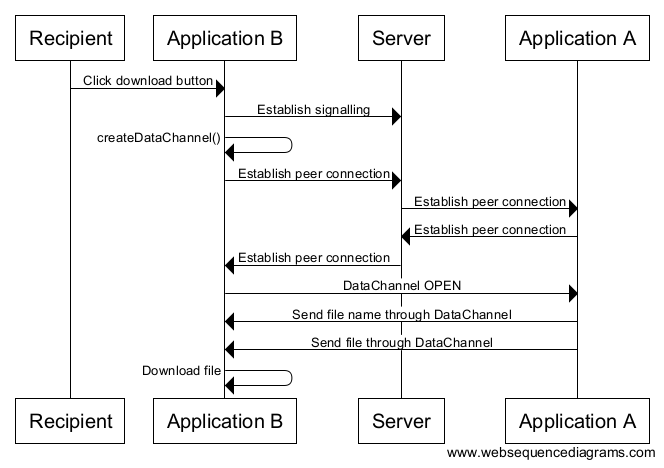
\includegraphics[scale=0.5]{file-sending-sequence-chrome.png}
			\end{figure}
			
			\begin{figure}[H]
				\caption{File sending sequence in Firefox}
				\centering
				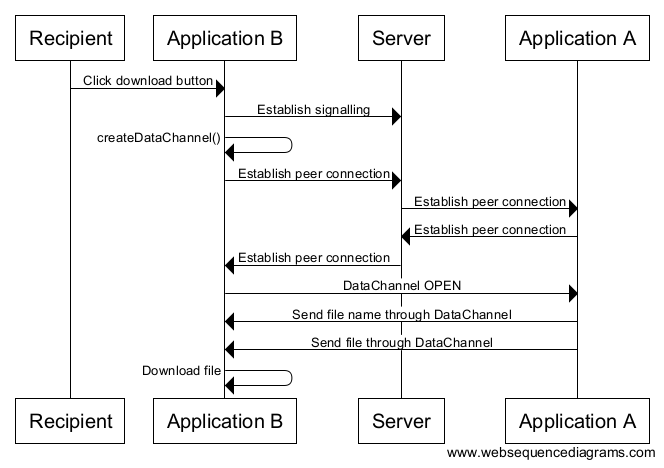
\includegraphics[scale=0.5]{file-sending-sequence-firefox.png}
			\end{figure}	
			
			\subsection{Media Streaming}
				\subsubsection{Audio}
				To convert a file into a Media Stream ready for adding to the peer connection, the application uses the HTML5 File and WebAudio API. It does this by loading the file into a FileReader object which returns an array buffer (fixed length array containing binary data) that is decoded by an instance of the WebAudio AudioContext. On decoding the data, it creates a source object from it which connects to a destination representing an output such as a speaker or a MediaStream. Once it has done so, the stream from the MediaStream object can be added to the peer connection after the offer has been received from the file recipient. Once the answer SDP containing the media parameters for this stream has been sent back and the peer connection is established, an event listener on the recipient application listens for the event signalling the addition of this stream and uses the HTML5 Audio API to create a new audio element which is appended to the html. The source attribute of this element is set to the incoming stream and the audio player is set to play automatically.
				
				It is important to note that the stream actually starts to play when it is created by the uploader as it is a "live stream" and if there is any latency issues between the two clients or if the recipient decides to pause the player, the stream will carry on and they will miss parts of it. To avoid the problems with live streaming, an alternative to this could be to make the recipient completely download the file from the uploader using RTCDataChannel before playing it using the HTML5 audio element. By doing so, they would be able to pause and control it. The problem with this is that it puts a limit on the size of the file that can the uploader can stream to a recipient as the RTCDataChannel has a size limit on what can be sent through, particularly in Chrome.

				\subsubsection{Video}
				I originally planned on also adding video streaming to the application. However, when I looked into this, the part of the MediaStream processing API drafted by W3C \todo{CITE} that would capture video as a stream has yet to be implemented by any browsers. Similar to how audio is captured, The captureStreamUntilEnded() function would return a MediaStream containing both the audio and video tracks of a file which could then be passed to the peer connection and played by a HTML5 video element on the recipient's application after the peer connection has been established. These issues could also potentially be avoided by downloading the file via RTCDataChannel before playing it with a HTML5 video element as it means the uploader would not have to convert the file to a media stream in order to transfer it to the recipient.
			
			\subsection{One-to-many peer connections}
			Switching to the Node.js implementation of the server allowed for one-to-many peer connections to be implemented with ease. To do this, the uploader instantiates new peer connections and adds them to an array which are then used to communicate with the recipients which only holds one peer connection (to the uploader). Each message sent via the signalling server contains the socket ID of the user it is from and the user it is destined towards, which is then extracted by the server and used to send messages to only their socket, this way no information can be exposed to anyone except for the user it belongs to. One of the big disadvantages of this is it places a larger amount of load on the uploader as they now have to maintain and search through an array of peer connections making the load increase with the amount of users. To reduce this, the recipient sends a message to the uploader signifying to close the connection and remove it from the array as soon as the recipient has downloaded the file. In the future, this functionality will also be added for when a MediaStream ends but currently the MediaStream API in Firefox or Chrome has no way of establishing when a stream has finished.
			 
			\begin{figure}[H]
				\caption{One-to-many peer connections}
				\centering
				\includegraphics[scale=0.5]{One-to-many.png}
			\end{figure}	
			
			\subsection{Data Aggregation}
				\subsubsection{Data Collection}
				In order to gather statistics on the peer to peer connections within a room, two new functions were created, one for streaming and one for downloading. These are called on the recipients application in order to collect information about the transfer of data. For the streaming data, the function utilised the WebRTC GetStats API\todo{CITE} which returns a raw data object containing information about the connection including the streams and data channels that exist within it. The function calls the getStats function and then extracts data from the resulting data object in a callback, this is then sent to the signalling server along with the room ID and the socket IDs representing the user at each end of the connection. In the download data gathering function, the getStats API was not used as it does not contain useful statistics about the DataChannel, instead a custom object was created that contained the amount of bytes that was sent through to the recipient in each chunk as well as the bytes received per second and the overall time taken. In both functions, this data is sent to the signalling server which then adds file meta-data to the statistics object such as size and type which is gathered when the file is initially uploaded. As Firefox doesn't require files to be chunked in order to send them, the download function cannot record how many bytes are sent per chunk or second as it relies on measuring how fast the chunks are sent, due to this the application in Firefox only records the time taken from when it sent the offer to when the file was downloaded. On the server, this information is logged to a file using a logging library called Winston that formats it with a time stamp. Winston is built to provide a simple interface to log to and query from multiple locations (or "transports"). Using this framework allows for the logging process to be easily scaled with the application if it was extended in the future.
				
				\subsubsection{Data Visualisation}
				To monitor the application, the data received from the recipient was also modelled using a data visualisation tool. There are a number of tools and libraries that enable developers to do this such as D3.js \& Charts.js. Initially, a pre-built data visualisation server built with node.js called Lightning-vis was chosen which uses a REST API to communicate with and send data to. This way after being sent to the signalling server, the data was able to be streamed to the data visualisation server and the connections in each room could be monitored in near real-time. Instead of directly interfacing with the REST API, a JavaScript API client library was chosen that obfuscates it and makes it easier to code against. Using this, the application created a lightning server session when each room was generated on the application and once a user started downloading or streaming, the data was posted to visualisations contained within this room. 
								
				\begin{figure}[H]
					\caption{Lightning Viz Session}
					\centering
					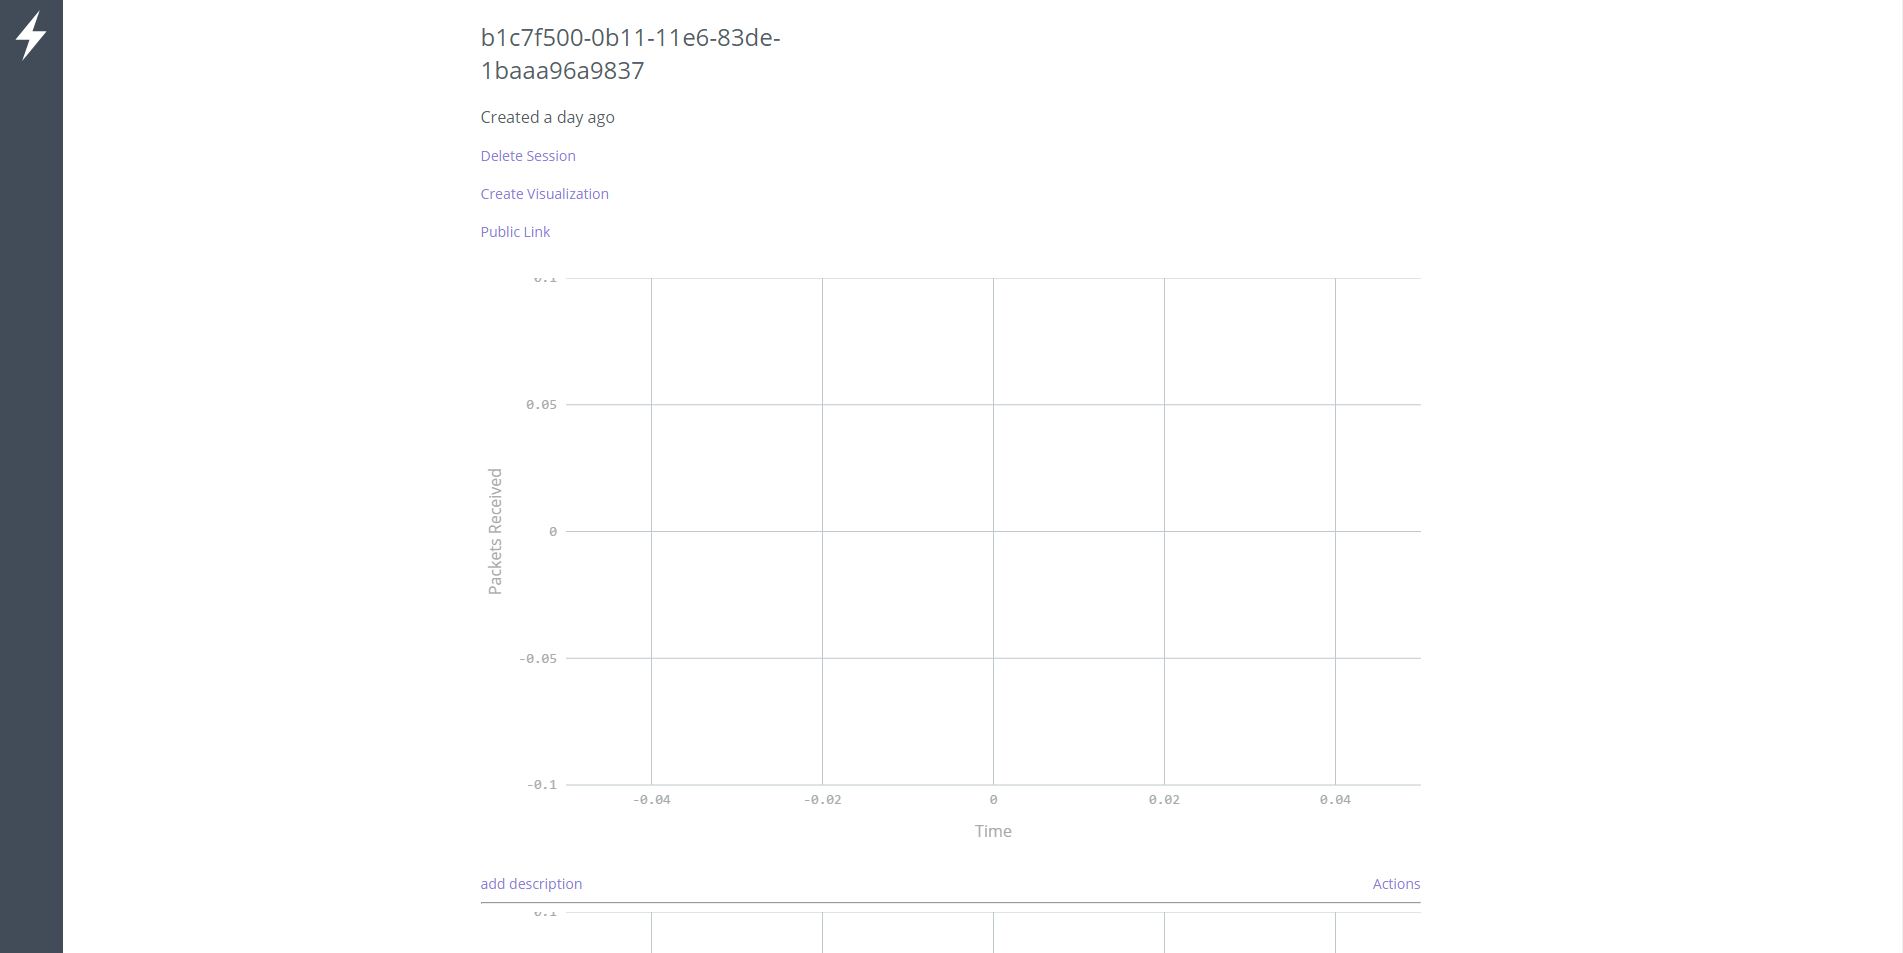
\includegraphics[scale=0.25]{lightning-viz.png}
				\end{figure}	
				
				However as the server and API client were being developed with, the limitations of the functionality became apparent. For example, once a visualisation was created within a session, only the initial data series that were created with it were able to be updated, this meant that new series could not be added to represent recipients as they joined and left the room. Another issue was that the JavaScript API client had not been updated since the REST API had changed and an endpoint had to be changed for it to work. Overall, it was decided that it would be better to approach data visualisation with a different library instead of expending any more time trying to make it work. 

				As an alternative, Lightning vis was replaced with a lightweight JavaScript library called smoothie.js that utilises the HTML5 canvas element to produce live streaming graphs. This library was implemented to add graphs to the uploader's application, enabling the user to see how fast the peers connected to them were either downloading or streaming the uploaded file. To do so, the signalling server was updated to forward these statistics on to the uploader. Using smoothie.js avoided the problem occurring with the lightning-viz server as it was now possible to add a series per recipient to the charts after they were initialized. However, one of the downsides of this was that now the data visualisation and processing is all handled within the application which presents two problems. First of all, it puts extra load on the application instead of passing it to a service built for this purpose (like lightning-viz) which is probably considerably more efficient at it and secondly by doing so, it means that only the uploader can view the visualised statistics for the room. Due to this, the solution should considered to only be temporary and refactored at a later point to use a solution such as the ELK (ElasticSearch, LogStash, Kibana) stack. Logstash is a tool that Winston can transport logs to and is used to centralize the aggregation of data, in combination with elastic search which searches and analyses this data and kibana for data visualisation, it would provide a better, more scalable solution.
				
				\begin{figure}[H]
					\caption{Smoothie.js Chart}
					\centering
					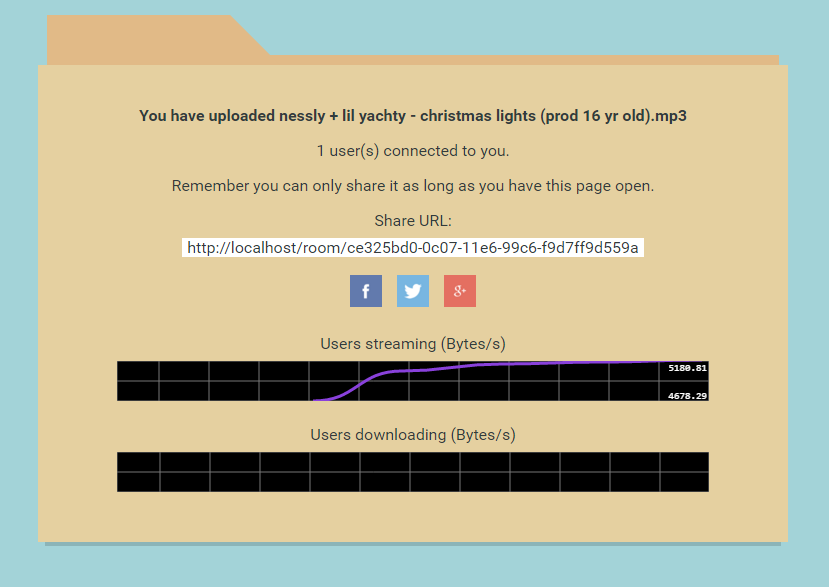
\includegraphics[scale=0.5]{smoothie-js.png}
				\end{figure}
			
		\section{Presentation}
			\subsection{Design}		
			\todo{GOOVERTHIS}	
				As design and usability was not a key part of my project, the design and structure of the web application was kept simple and clean in order to minimise time and effort spent on it and to emphasise the sole purpose of the project. However, the design of the application was still something that needed to some time dedicated to it as having a poorly designed application limited how easily I could test it especially with the lack of unit tests.
				
				\begin{figure}[H]
					\caption{Iterations of Design}
					\centering
					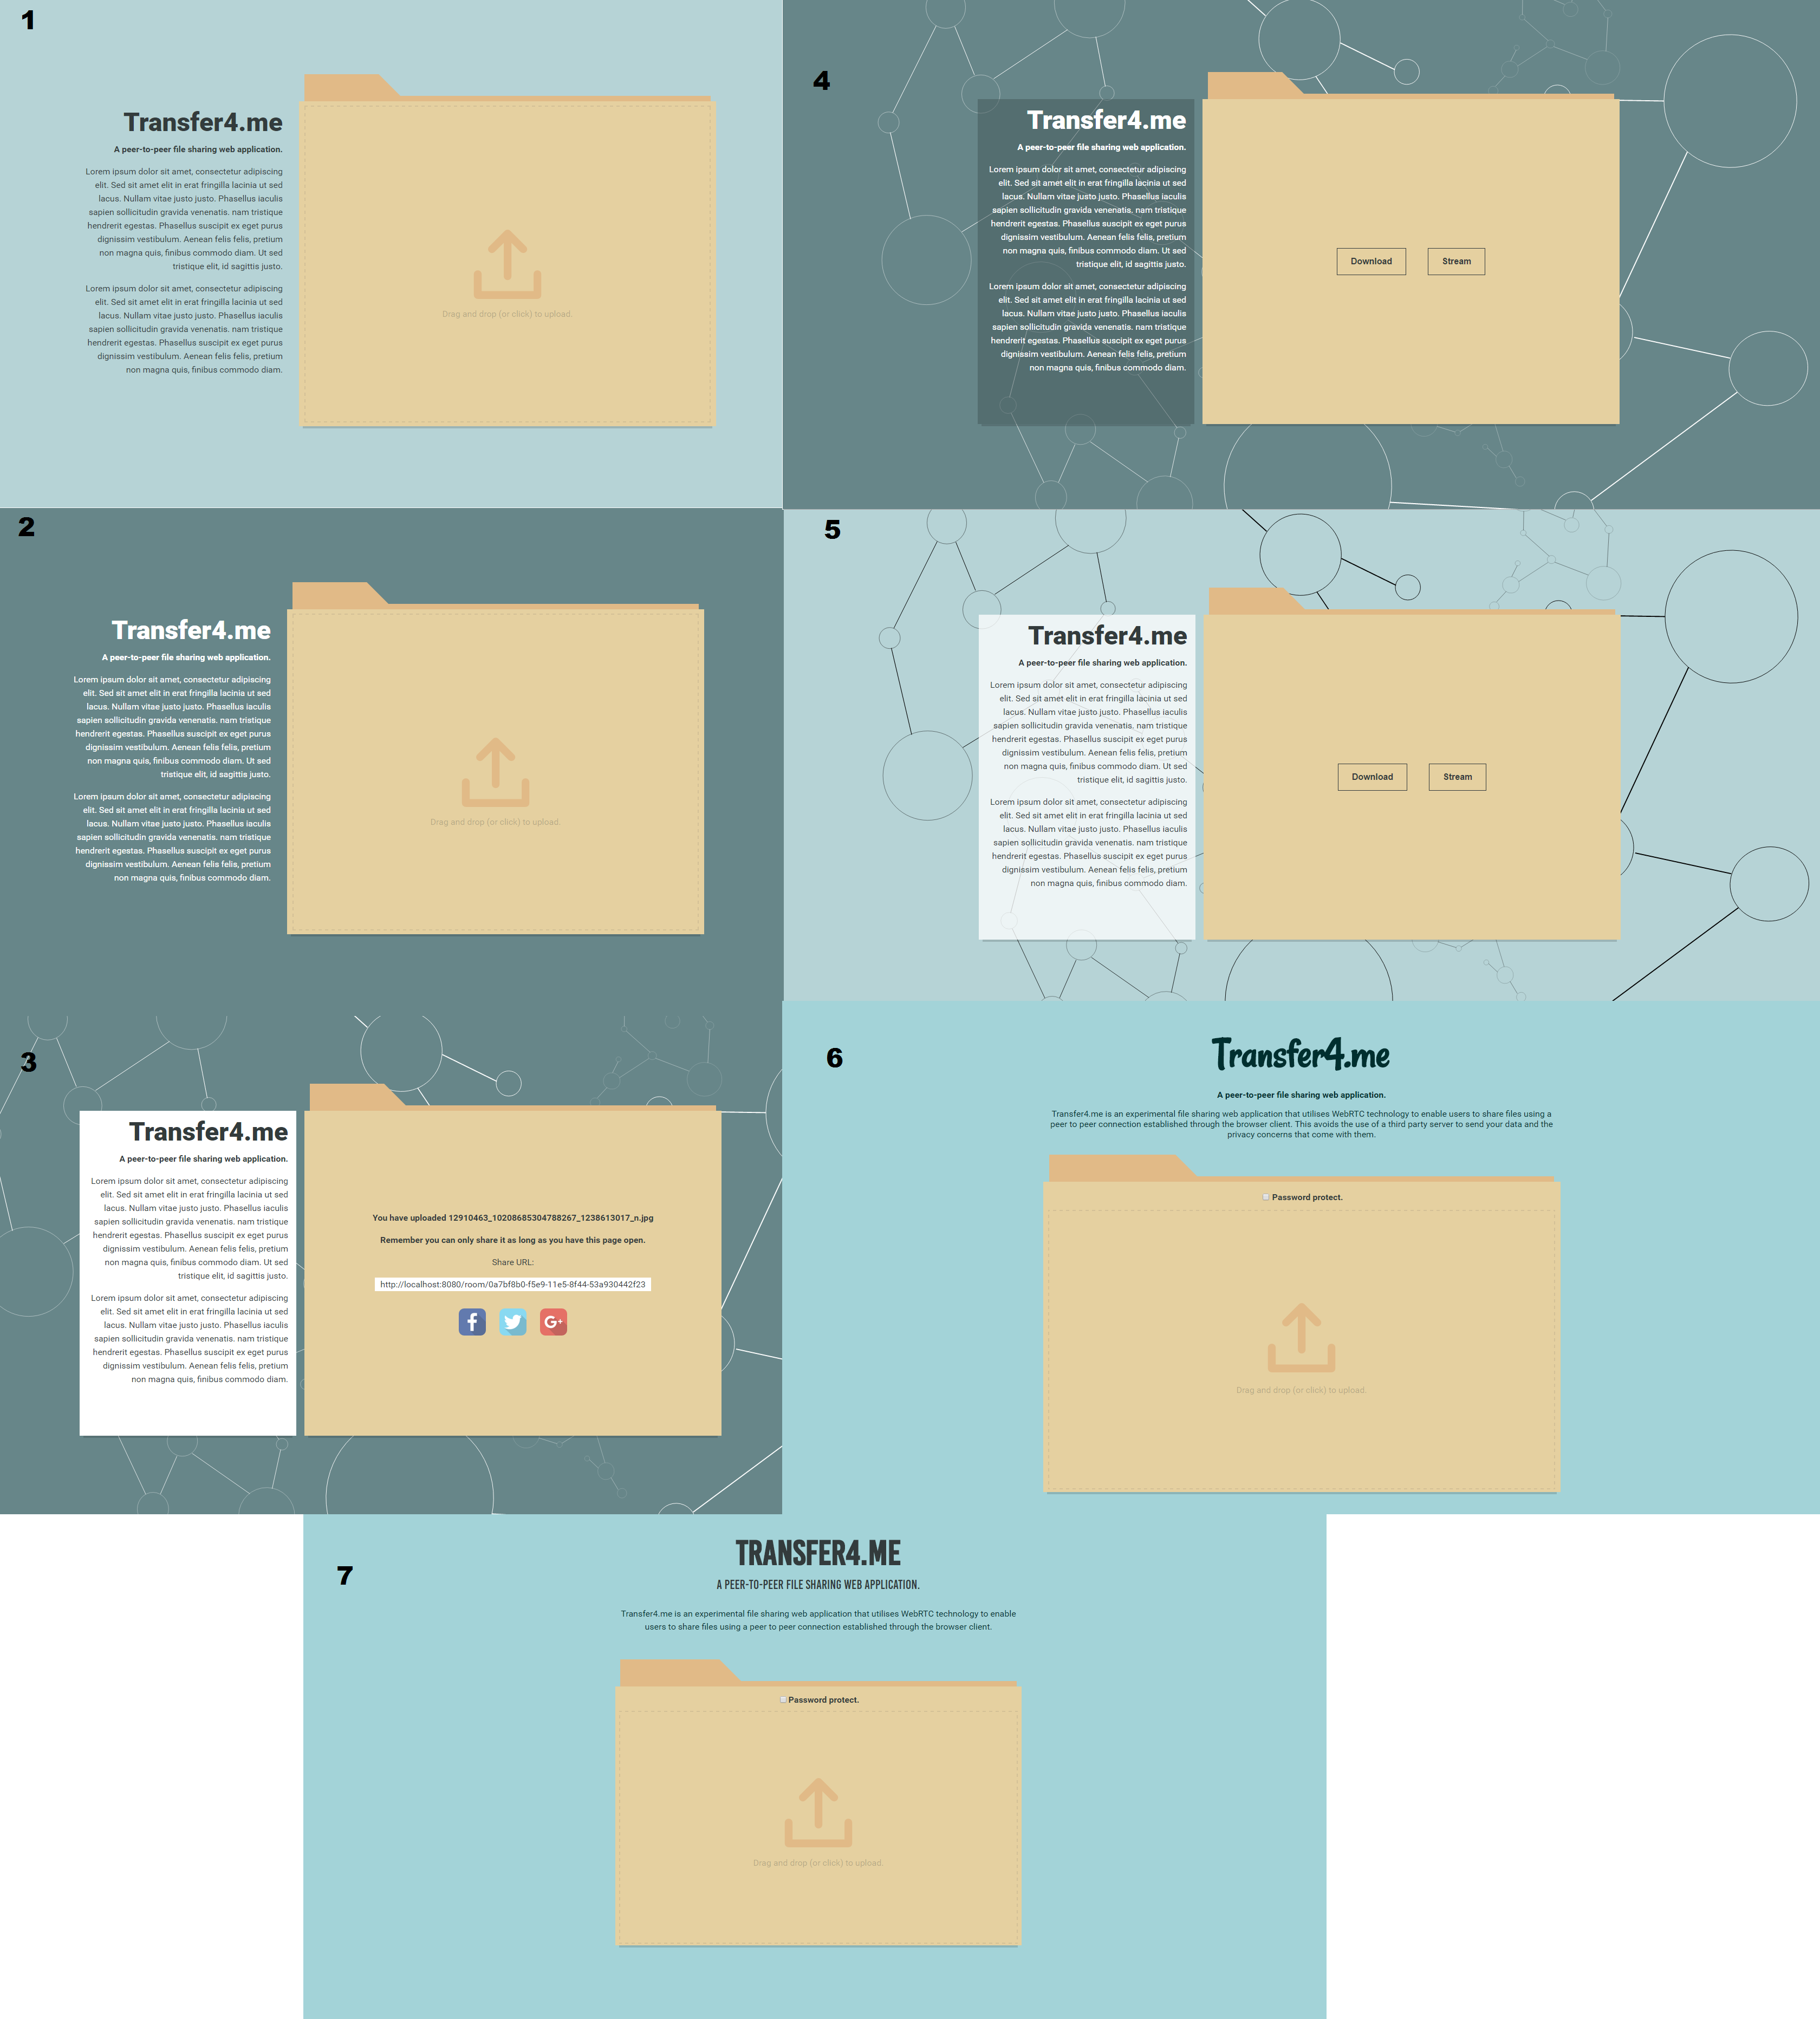
\includegraphics[scale=0.15]{design.png}
				\end{figure}
				
			\subsection{App.js module}
			Initially to develop the code that would present and manipulate the state of my application, JavaScript frameworks such as Backbone.js and Angular.js were looked into. However, this seemed unnecessary as the the states of the application were relatively simple. Instead, a basic set of functions that put the application into these states was developed and added to the app.js module. These functions manipulated the Document Object Model on the page using JQuery where possible and vanilla JavaScript where it couldnt be used. To transition into these states, these functions also asynchronously called functions from the lower level JavaScript modules in order to initiate a connection to the WebSocket and set up in preparation to receive an offer for a peer connection.
		
		\section{Authentication}
		To add basic authentication to the application, an option was added to the file upload state of the application that enabled the user to add a password to their "room". In the background, this worked by sending a password field through with the POST request to create a room if the password option was selected. A password would then be generated by the server and passed back to the client to present to the user. When a recipient then attempted to join a passworded room without a password cookie, they would be served a password page. This password page retrieves the password from the recipient and sends it in a POST request to the server, checking it against the room's password to validate it. If it is correct, a cookie containing the password is added to the response and the user is redirected to the room page, again checking to see if the cookie exists with the correct password. The reason for the intermediary password page is that if the password was asked for on the main room page, a user with experience of web development could easily bypass this and join the room without being authenticated.
		
		\section{Other Technologies}
			\subsection{JavaScript Build Tools}
			In order to streamline the process of developing with JavaScript I used a tool called Browserify. As explained earlier, Browserify is a dependency management tool that allows you to use node.js modules in the browser as well as allowing you to modularize JavaScript to produce a more structured application. However, to compile the bundle of dependencies together, a command line interface is used. This can be done manually but starts to become inefficient when code is being changed constantly. An alternative to doing it manually is to automate the process using a task runner such as Gulp. Gulp is essentially a task runner that allows developers run all of the pre-processing needed to build their compile static resources. In order to automate the Browserify process, I found a gulp task that uses a JavaScript library called watchify that monitors JavaScript for changes and recompiles the bundle when it does. I was then able to run this gulp task through the command line whenever I was developing so that I did not constantly have to run Browserify myself. In the future, I could also use gulp for other tasks, for example if I refactored the application's css to use sass instead, I could create a task that watches the sass files for changes and automatically compile them.
			
			\subsection{Development Environments}
			I used WebStorm, an integrated development environment for JavaScript. I chose it because of the massive range of functionality I could utilise as opposed to basic text editors such as sublime. An example of this functionality was that I was easily able to run and specifically debug processes such as the browserify gulp task and the node.js signalling server through it which saved me a lot of time that I would have spent setting up a third party node.js debugger. It also allowed me to spot syntactic and semantic errors as I was writing the code and do things such as refactor names of functions without crawling through the rest of the code to see where it is used.
			
			\subsection{Git}
			Throughout the development process, I regularly committed code to my GitHub repository using the git command-line interface. This was a great habit to get into as it allowed me to track and log my work throughout as well as prevent any risk of accidental data loss or overwrites that would almost definitely have occurred from using a USB stick or even a cloud service like dropbox. it let me easily switch from one development platform to another without any trouble which was extremely important as I was in and out of university most days. This habit also spilled over into other modules as I now have a GitHub repository for each that contains all of the assignment work I have done for them. Using GitHub also allows me to expose my work with potential contributors as it is open-source as well as employers as an example of my abilities. 
			
			\subsection{Amazon Web Instances}
			Amazon Web Services allowed me to quickly spin up and destroy virtual Ubuntu server instances to host the application on. In the end, I also linked this server with a domain address in order to provide a public interface into the application. However, choosing the free micro server instance that Amazon provide could potentially bottleneck the application. In order to scale the application, the server would eventually have to be upgraded to a better but more costly server instance.			

	\chapter{Testing}
		\section{Automated Testing}
			In order to test the server functionality, I used a Node.js testing framework called Mocha. Test cases were created for each endpoint of the API and most of the WebSocket functionality. Mocha does this by running each test within an asynchronous callback. Within each of these test cases, the correct application state is set up by mimicking the real application's requests to the server. Once it has reached this state, a request is sent to an endpoint using the supertest.js library which then uses a callback to listen for the response. Once it has received this, supertest.js is able to compare the response of the request with the expected results through assertion functions. To test WebSockets functionality, the socket.io client was used to connect to the server like the application would, from this point signals could be sent through the server to another socket. By testing each aspect of the server's functionality in isolation, it makes the code easier to understand, maintain and extend whilst by preventing bugs from being missed and ensuring that each function is doing what it is supposed to.
		
		\section{Manual Testing}
			Due to the lack of a unit testing framework for client-side JavaScript, I was unable to write unit or integration tests for the browser modules. In order to overcome this, manual testing was emphasised throughout the development process. Every time functionality was added or changed, it was thoroughly manually black-box tested with the different possible use cases. To automate this process to an extent, the iMacros Chrome extension and the Selenium WebDriver plugin for Firefox were also investigated. These tools allow testers to create scripts that go through the flow of the application. iMacros ended up being abandoned as it was failing too often but with Selenium in Firefox, test cases were made for downloading and streaming. An end to end test case was unable to be scripted as Selenium couldn't seem to handle using the file element to upload a file. A Chrome application called Postman was also used to black box test the endpoints of the API. This application allows for test cases consisting of HTTP requests to be created and fired against the server. Through this, I was able to test each endpoint in isolation from the client side application. 
		
		\section{Stress Testing}
		In order to load test the application, it was put under varying amounts of stress by changing factors such as the size of the file and the amount of concurrent users downloading or streaming the file and analysing the statistics from the log file. For the download test cases, the time taken from the offer being sent by the recipient to the time the file had been successfully downloaded was used as the benchmark. As streaming can't be measured in terms of how long it takes, average throughput (bytes per second) was used as the benchmark and the amount of users streaming the file became the variable. The download test cases were ran 3 times per amount of users per file size and the stream test cases were ran once per amount of users per file size. It is important to note that all of these tests were ran on the same browser on the same device so results could be limited by this and users may not have been truly concurrent downloading smaller files even with browser automation tools such as Selenium as the download could have occurred too fast. To improve this, the tests could be ran on separate devices concurrently in order to minimise the effect that it could possibly have on the results.
		
		\subsection{Discussion of results}
			\subsubsection{File Transfer}
			\begin{figure}[H]
				\caption{Average time taken to download a file}
				\centering
				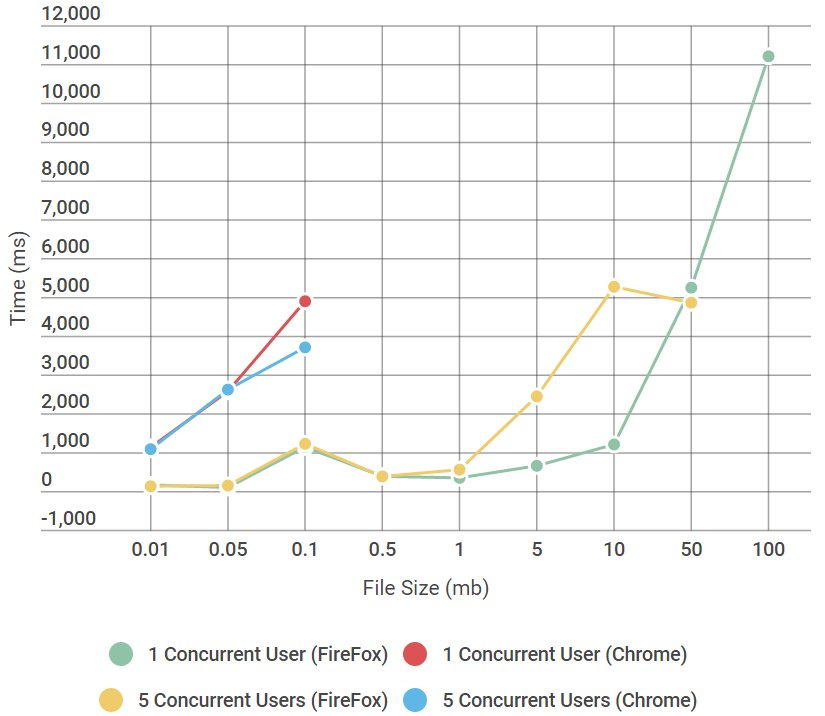
\includegraphics[scale=0.5]{download-chart.png}
			\end{figure}
			\begin{figure}[H]
				\caption{File download failures}
				\centering
				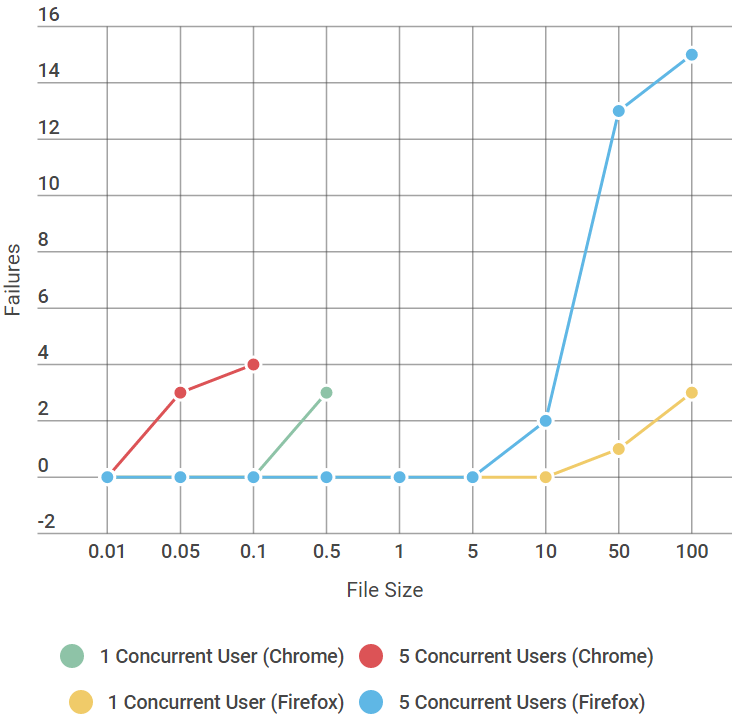
\includegraphics[scale=0.5]{download-failures-chart.png}
			\end{figure}
		
			By analysing figure 6.1, it can be seen that Firefox was able to download files of much larger size than Chrome. This is most likely due to the limit on throughput (in terms of bytes per chunk) Chrome imposes. It can also be noticed that the larger the file size, the more failures occurred in Chrome. This implies Chrome also limits the overall amount of data that can possibly be received through the RTCDataChannel as once the uploading peer had sent a certain amount of chunks, the recipient application would stop receiving them even though they were still being sent. 
			
			Both these factors suggest that Firefox is currently a more consistently successful browser for using RTCDataChannel with. This could be because Firefox has an official implementation for handling file transfers through the data channel. On the contrary, the failures in Chrome could be explained by both the stricter WebRTC limitations Chrome has implemented and the bypass I had to implement in order transfer files.
			
			Early in figure 6.1, there is an outlier where Firefox took longer to download a file at 0.1mb than it did at 0.5mb. This was particular unusual as it didn't occur in isolation as every repeated test with both 1 user and 5 users gave this average time. As it was replicable, the result could have been due to an issue with the file I used to run the test on.
	
			\subsubsection{File Streaming}
			\begin{figure}[H]
				\caption{Average streaming throughput}
				\centering
				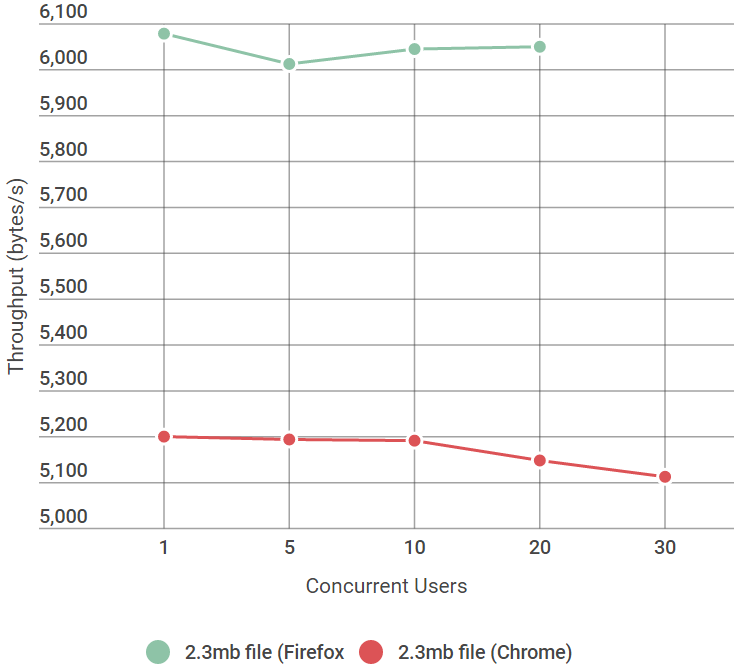
\includegraphics[scale=0.45]{streaming-chart.png}
			\end{figure}
			\begin{figure}[H]
				\caption{File streaming failures}
				\centering
				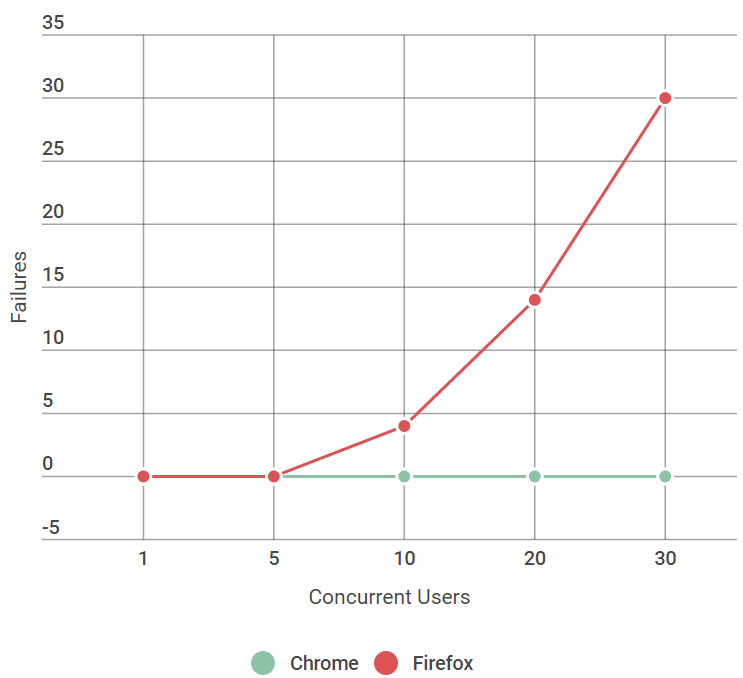
\includegraphics[scale=0.45]{stream-failures-chart.png}
			\end{figure}
			
			Figure 6.3 shows that Firefox streams data at a higher average throughput than Chrome. One explanation for this could be that Firefox streams media at a higher quality than Chrome does. This could also explain why Firefox incurs more failures as the amount of streaming users increases as seen in figure 6.4 with Firefox being limited to around a maximum of 5-6 users streaming at a time. This limit on the amount of users and the higher average throughput supports the idea that Firefox has a higher stream quality that is less scalable with more users. Another explanation for the higher average throughput could just be that Chrome uses and sends less meta data per byte of data streamed and the limit on the amount of users could have been because of the fact that all of the streamers were ran from the same browser instance on the same device and Firefox could have a limit on incoming streams.
		 	
			Due to the uncertainty surrounding this difference in average throughput, a better way of analysing the data is to look at the amount of variation within each browser's series as the amount of users increases. Looking at it this way, it can be seen that Chrome has a more consistent throughput than Firefox as the amount of user's scale until the users becomes too high and the throughput starts to decrease. Chrome also has no failures as users increase whereas Firefox increases dramatically until all of the streaming completed failed at 30 concurrent users.
			
			\subsubsection{Summary}
			Chrome seemed to perform better at streaming and Firefox seemed to perform better at downloading. These results were expected to an extent due to the limitations and problems encountered when developing with WebRTC in each browser, particularly with Chrome's file transfer limitations. Overall, it is worth mentioning that the application performed better than expected especially with so many users considering WebRTC is a technology that was specifically designed for one-to-one real-time communications as opposed the purposes it was used for in this application. Unless W3C start to define standards for this or a new technology arises that is specifically designed for it, there will always exist limitations to how well it can be implemented. That said, there is functionality that can be added such as many-to-many connections that can help reduce the effect of these limitations.
		
	\chapter{Review \& Reflection}	
		\section{Background Research}
		The background research that was investigated prior to the development of the project definitely influenced the application and the technologies it used. In particular, the research into WebRTC provided the basis on which peer to peer connections could be established through the browser. Without this, the project would not have been possible as there is no other technology enabling this.
		
		The research into network architecture would have been more relevant to the development of the application had the many-to-many peer connection functionality been implemented as the network topology would have been relatively more complicated. However, it was instrumental in my understanding of the context in which technologies such as WebRTC work and thus how my project would be achieved.
		
		Last of all, research into the current file transfer solutions could have covered peer-to-peer solutions more thoroughly as opposed to traditional client-server solutions as they would have provided more of a relevant insight into the technology and concepts that could have potentially been replicated in this application. On the other hand, by researching these traditional solutions, it gave substance and explanation to the motivation behind the project.
		
		\section{Specification}
		Due to limitations within the technologies that were being using, the deliverables that came out of the project were slightly different from the ones set out by the specification. For example, the signalling server had to be re-factored to use Node.js instead of Java due to problems with the WebSockets implementation. As a result of changes like this, the estimated schedule of activities in Figure 3.1 did not reflect the actual time line of events. However, this was expected to occur as the application was relatively experimental and project estimation is inaccurate most of the time.
		
		By the benchmarks set up in the quality analysis section of the specification, the application would be considered a success. Although, there were a few things that it did not achieve such as the many-to-many network due to a lack of time. This also resulted in not being able to compare the performance of the many-to-many network with the one-to-many network. In the end, the application was not compared to other services such Dropbox and Google Drive as it would not be possible to replicate the superior servers and environment they are run on. The signalling server was also not load tested as this is unnecessary unless the application was running on a production server. Instead, the signalling server underwent unit and integration tests.
		
		\section{Methodology}
		Throughout the project's timeline, I was able to maintain an iterative and evolutionary approach to software development. However, there were obstacles to this such as the lack of a unit testing framework for JavaScript in the browser. This stopped me from using processes such as test-driven development which was a big part of the planned iterative cycle. As a result, the process was adapted to use manual black and white box testing as the main means to test the application. Although this was not as strict as using formal unit tests, I feel like it did make the process less cumbersome and it was a good example of how an iterative methodology should adapt to unpredicted changes like this.
		
		One of the limitations of implementing an iterative approach like this was that development was often focused on meeting immediate smaller goals such as establishing a one-to-many network without thinking about the long term goals such as implementing a full many-to-many network. This resulted in code that would work for the current features but would not necessarily be very extensible, requiring a lot of refactoring to fix it.
	
		\section{Limitations \& Improvements of the application}
			\subsection{Network Structure}
			Currently the application supports one-to-many peer connections but this can become a problem when too many recipients connect to a file uploader. An efficient way to avoid overloading the uploader would be through maintaining a pool of nodes that have already downloaded the file (or seeds) on the signalling server from which incoming peers can download the file with each of these seeds maintaining their own an array of peer connections. This way, a limit can be set in order to prevent one seed from becoming burdened with too many recipients. Once each seed has reached its limit, it would alert the signalling server and other incoming peers would be redirected to download or stream from another seed. Once these incoming peers download the file, they become seeds themselves, forming a new network of peers. When every seed in the pool is saturated with a peer, the rest can then be enqueued via a FIFO queue and wait for a seed to become free. This approach would ensure that the file could propagate to new incoming peers even when the the original uploader has disconnected from the room as long as there was always one seed. One constraint with implementing this in my application is that only the downloaders could be considered valid seeds as they are sent the actual file whereas streamers would only be sent an audio stream of it.
			
			\begin{figure}[H]
				\caption{Many-to-many peer connections}
				\centering
				\includegraphics[scale=0.5]{many-to-many.png}
			\end{figure}	
			
			This structure would eventually form a network topology similar to a tree network in which multiple nodes spawn from one node and eventually develop their own network of sub-nodes and so forth. Due to this structure, the network would be relatively easy to maintain and scale as each node would only needs to maintain the connection between it and it's sub-nodes. It would also provide a higher level of redundancy as the signalling server could be used to reconnect nodes to another seed if there is a failure with the original. The downside of this is that it puts more reliance and load on the server to organise the network, which is problematic if the signalling server crashes.
			
			\subsection{JavaScript standards}
			As JavaScript was relatively new to me at the beginning of this project and it ended up being the language used throughout the full stack, the standard of the code could most likely be improved. An example of this is how callback functions were utilised instead of using the concept of promises. Promises are essentially objects that represent the potential result of an unfinished asynchronous operation. When these objects are created, they are initially empty but become fulfilled when the operation has finished or rejected if the operation fails. To use a promise, the code that is to be executed after the asynchronous operation is to be passed through to one of two functions called then() for successful results and catch() for failed results which are chained on to the end of the call to the asynchronous operation. This works because both functions return a promise which can be pipelined through each other. The major benefit of this is that by making the asynchronous operation an object, it can be passed around as a first class citizen whereas if a callback was used, this wouldn't be possible.	

			\subsection{Authentication Encryption}
			At the moment, the authentication process is relatively simple. In order to improve security, the generated password should be hashed on the server and password validation should occur by hashing the incoming password and comparing it to the version on the server. Although this isn't a major issue as the server only keeps the password for as long as the room exists and not in a database, if it ended up being compromised it would mean that the hacker would potentially have access to every passworded room. 
			
			\subsection{HATEOAS}
			HyperText As The Engine For Application State (or HATEOAS) is a concept within the REST architecture that dictates a client using an API should be able to navigate throughout it with little knowledge of it. This would be achieved by ensuring the response of every API request sends back a list of other possible endpoints that can be used on the resource for the client to use. For example, GET /room/{roomId} would return the URIs /room/{roomId}/fileType and /room/{roomId}/password in the response. The benefit of this is that if the URI structure of the API changes, it does not break the client as they would be using the URI returned from the server as opposed to a hard-coded URI.
			
	\section{Conclusion}
		Although this project has shown that WebRTC has potential to provide consumers with an alternative means of transferring data over the internet, it is limited as WebRTC's primary purpose is enabling one to one real time communication. Due to this, WebRTC does not have the native means to effectively scale and transfer data to large amounts of people. This results in the application implementing this technology having to handle this, resorting to less efficient hacks and bypasses being used in order to make it work. In order for peer to peer data transfer through the browser to be considered a full alternative to current solutions, a specific technology would have to created that was able to deal the with optimisation and scalability concerns shown by this project at a browser level. This being said, WebRTC presented a novel opportunity to work with concepts like this and it could definitely be utilised to supplement current solutions. For example, the ability to stream audio files from one peer to another could be incorporated into a platform such as Spotify in order to ease load on servers. 
			
					
	\begin{thebibliography}{20}
		\bibitem{Unstructured P2P Diagram}
		An Unstructured Peer-To-Peer Overlay Network. Available: http://www.hindawi.com/journals/jcnc/2012/485875/fig1/. Last Accessed 6 Nov. 2015.
		\bibitem{P2P overlay networks}
		Eng Keong Lua Crowcroft, J. ; Pias, M. ; Sharma, R. ; Lim, S.. (Second Quarter 2005). A survey and comparison of peer-to-peer overlay network schemes. Communications Surveys \& Tutorials, IEEE. 7 (2), 72 - 93.
		\bibitem{Hybrid P2P network}
		Yang, Beverly; Garcia-Molina, Hector (2001). Available: http://infolab.stanford.edu/~byang/pubs/hybridp2p\_long.pdf. Very Large Data Bases. Last Accessed 06/11/2015.
		\bibitem{P2P Security Issues}
		Schulzrinne, et al. (February 2010). Security in P2P Realtime Communications. Available: https://tools.ietf.org/html/rfc5765\#section-7.2. Last accessed 05/11/2015.
		\bibitem{Tree Topology}
		JOHAN GRONBERG, ERIC MEADOWS-JONSSON . (2014). Tree topology networks in WebRTC. Available: http://publications.lib.chalmers.se/records/fulltext/202811/202811.pdf. Last accessed 12/11/2015.
		\bibitem{Supernodes}
		Jan Sacha. (2009). Exploiting Heterogeneity in Peer-to-Peer Systems Using Gradient Topologies. Available: https://www.scss.tcd.ie/publications/tech-reports/reports.10/TCD-CS-2010-06.pdf. Last accessed 12/11/2015.
		\bibitem{CSA Top Threats}
		Cloud Security Alliance. (2013). The Notorious Nine Cloud Computing Top Threats in 2013. Available: https://downloads.cloudsecurityalliance.org/initiatives/top\_threats/The\_N\\otorious\_Nine\_Cloud\_Computing\_Top\_Threats\_in\_2013.pdf. Last accessed 09/11/2015.
		\bibitem{PRISM}
		Greenwald, Glenn; MacAskill, Ewen (June 6, 2013). "NSA Taps in to Internet Giants' Systems to Mine User Data". The Guardian.  Last accessed 05/11/2015.
		\bibitem{IPB Encryption}
		Andrew Griffin. (2015). Investigatory Powers Bill could allow Government to ban end-to-end encryption, technology powering iMessage and WhatsApp. Available: http://www.independent.co.uk/life-style/gadgets-and-tech/news/investigatory-powers-bill-could-allow-government-to-ban-end-to-end-encryption-technology-powering-a6725311.html. Last accessed 09/11/2015.
		\bibitem{WeTransfer Storage Time}
		WeTransfer. How long are my uploads available to download?. Available: https://wetransfer.zendesk.com/hc/en-us/articles/202603916-How-long-are-my-uploads-available-to-download-. Last accessed 05/11/2015.
		\bibitem{WeTransfer AWS Case Study}
		Amazon Web Services. WeTransfer Case Study. Available: https://aws.amazon.com/solutions/case-studies/wetransfer/. Last accessed 05/11/2015.
		\bibitem{Amazon Social Engineering}
		Daniel Cooper. (2016). Amazon accused of handing out its users' personal data. Available: http://www.engadget.com/2016/01/25/amazon-social-engineering-hack/. Last accessed 01/05/2016.
		\bibitem{WebRTC Security Study}
		N/A. A Study of WebRTC Security. Available: http://webrtc-security.github.io/\#4.3. Last accessed 05/11/2015.
		\bibitem{Google WebRTC Release}
		Harald Alvestrand. (2011). Google release of WebRTC source code. Available: http://lists.w3.org/Archives/Public/public-webrtc/2011May/0022.html. Last accessed 29/10/2015.
		\bibitem{W3C WebRTC Definition} 
		Adam Bergkvist, Daniel C. Burnett, Cullen Jennings, Anant Narayanan (until November 2012). (2011). WebRTC 1.0: Real-time Communication Between Browsers. Available: http://www.w3.org/TR/webrtc/. Last accessed 29/10/2015.
		\bibitem{WebRTC browser support}
		Available: http://iswebrtcreadyyet.com/. Last accessed 30/10/2015.
		\bibitem{Mozilla Web API}
		Mozilla Web API. Available: https://developer.mozilla.org/en-US/docs/Web/API. Last accessed 30/10/2015.
		\bibitem{JSEP}
		Justin Uberti. (2011). Javascript Session Establishment Protocol (JSEP). Available: https://lists.w3.org/Archives/Public/public-webrtc/2012Jan/att-0002/JavascriptSessionEstablishmentProtocol.pdf. Last accessed 11/11/2015.
		\bibitem{WebSockets}
		Fette \& Melnikov. (2011). The WebSocket Protocol. Available: https://tools.ietf.org/html/rfc6455. Last accessed 12/11/2015.
		\bibitem{SDP Over WebSockets}
		S. Nandakumar, C. Jennings. (February 12, 2014). SDP for the WebRTC. Available: https://tools.ietf.org/id/draft-nandakumar-rtcweb-sdp-04.html. Last accessed 01/05/2016.
		\bibitem{WebRTC Data Channel Establishment Protocol} 
		Jesup, et al. (2015). WebRTC Data Channel Establishment Protocol. Available: https://tools.ietf.org/html/draft-ietf-rtcweb-data-protocol-09. Last accessed 12/11/2015.
		\bibitem{TDD Diagram}
		Available: http://www.agilenutshell.com/assets/test-driven-development/tdd-circle-of-life.png. Last accessed 09/11/2015.
	\end{thebibliography}

\end{document}          
